\documentclass[10pt, letter]{article}
\usepackage{graphicx}
\newcommand{\bigO}{\ensuremath{\mathcal{O}}}
\usepackage[center]{caption}
\newcommand{\doctitle}{%
Computational Creativity/Modeling and Design}
\usepackage{textcomp}
\usepackage{listings}
\usepackage{comment}
\usepackage{fancyvrb}
\usepackage[margin=1in]{geometry}
\usepackage{booktabs}
\usepackage[usenames,dvipsnames]{color}
\usepackage{hyperref}
\usepackage{algorithm}
\usepackage{algpseudocode}
\hypersetup{
  colorlinks,
  citecolor=Violet,
  linkcolor=Black,
  urlcolor=Blue}
  
\begin{document}

\title{Poetry Framework: Recognize Generate and \textsc{Understand} Poetry}
	\author{Arvind Krishnaa Jagannathan, Greg Cobb,
	Michelle Scott, Sonal Danak 
	\\[0.5cm] \textbf{\doctitle} \\
	\textsc{\textbf{Deliverable \#3:}} \date{}
	}
\maketitle
\thispagestyle{empty}
\section*{Description of the current system}
Our current working system essentially consists of 3 parts:
\begin{enumerate}
\item Two parsers - one for parsing each line of the CMU pronunciation dictionary (CMUDict) \cite{cmudict} and storing it to a database, and the other for parsing the poems entered or typed in by the user interacting with our current system.
\item Utility functions - Simple functions such as checking if two words rhyme with each other, getting the number of syllables in a word, generating a list of words rhyming with a given word and many more to be implemented in the future.
\item Recognition Element - to recognize if the text input is a haiku, limerick or a couplet.
\item User Interface - for the purpose of the demo.
\end{enumerate}
\subsubsection*{Parsers}
\subsubsection*{CMU Dictionary Parser}
The CMU Dictionary Parser is a one time pre-processor which reads each line of the CMUDict and stores the following information into a table in our MySQL database:
\begin{enumerate}
\item The word

\item The pronunciation symbols (phonemes and syllables) corresponding to the word

\item The last syllable of the word (this is just to save time so that the list created from step 2 need not be traversed again and again just to check if two words rhyme)
\end{enumerate}

We implemented this parser because the CMUDict does not provide any API to access its data quickly. It is simply a large text file, and we realized that the cost of scanning this text file every time we need to lookup a word is far greater than a database lookup.
\subsubsection*{Poetry Parser}
When provided with a piece of text, our system aims to identify whether the text falls into one the following categories of poems: haikus, limericks and couplets. For this purpose, the parser module tokenizes the text in two ways. First, it counts the number of lines in the text (the number of lines in a poem is often essential to identifying its category). Another functionality of this module is to extract the last word from an indicated line belonging to the text. The purpose of this extraction is to enable the system to identify whether there exists a certain rhyme scheme pertaining to the text. A rhyme scheme is another essential element in identifying the category of a poem. The input to this module is the piece of text that we wish to identify and the results are utilized by the recognition module that finally categories the text.

\subsection*{Utility Functions}
We would obviously require a lot of utility/helper methods to assist in this project. At this stage, we have written a few simple ones, and have utilized NLTK (Python’s Natural Language Toolkit)\cite{bird2009natural} to find the number of syllables in a given word. Here are the two simple methods which we have implemented:
\begin{enumerate}
    \item Check if two words rhyme with each other: Right now we simply assume that two words rhyme with each other if their corresponding symbols in the CMUDict have the same ending. Obviously this may not cover complex rhymes, or words twisted in their pronunciation to fit into a rhyme scheme (as is popular in rap), but it is a good starting point.
    \item Generate a list of rhyming words for a given word: Here we get the symbol list from CMUDict for the word given as input and lookup a list of words in the CMUDict which also have the same ending (very similar to 1). By default we restrict the number of words returned to 10, but by adjusting a parameter to the input, we can generate as many rhyming words as required.
\end{enumerate}

\subsection*{Recognition Element}
The recognition element currently implemented is a naive version of what we would like to achieve in the end. As of now, it is able to recognize if the input given to it is a haiku, limerick or a couplet poem. The recognition element achieves this by comparing the text in each line of the input to the rules governing those poems (which we have described in Deliverable 2). For the purpose of completeness, here is a brief description of how we identify each of these poems:
\begin{enumerate}
\item Haiku Poem: We check if the input has exactly 3 lines (we use the newline character as the delimiter). If it does, we break down each line into constituent words (by assuming that words are delimited by a space). For each word we look up their syllable count in the CMUDict and thus creating an in-memory representation of the number of syllables in each line (say <n1,n2,n3>). Once the input is exhausted, we compute the total number of syllables in the input (say n). n1, n2, n3 need to be 5,7 and 5 respectively (and of course the total will be 17). If the input violates even one of these conditions, it will be flagged as not a Haiku.

\item Limerick Poem: The input text needs to have exactly 5 lines. If it does, we get the last word for each line. If the last words of lines 1,2 and 5 rhyme and the last words of lines 3 and 4 rhyme, then we declare that the input is a Limerick. Again, failing any of the conditions immediately will disqualify the input from being a Limerick.

\item Couplet Poem: This is probably the simplest of the three to recognize. If the input has two lines and the last words of those two lines rhyme with each other then the input is a couplet; failing which it is not.
\end{enumerate}

The recognition element will take an input text and run it against each of the above 3 rule-sets and will return the first matching category of poetry it belongs to. If none of the above categories match the recognizer throws a popup giving this information.
\subsection*{User Interface}
As of now, the functional components of the user interface consists of a main menu, from which the user can select either to find a poetry type within a piece of text (which right now is the simple recognizer) and associated windows for each of the menu items in the main menu.
    However, the main interface element is the recognizer element, where a user can type in text, or choose a text file; text from this would be placed in a text area and once the user clicks on the “Search” button, the recognition element will check if the input belongs to one of the three types of poems we have defined. They user interface is presented in Figures \ref{screen1} and \ref{screen2}.
    
\begin{figure}[ht]
  \centering
    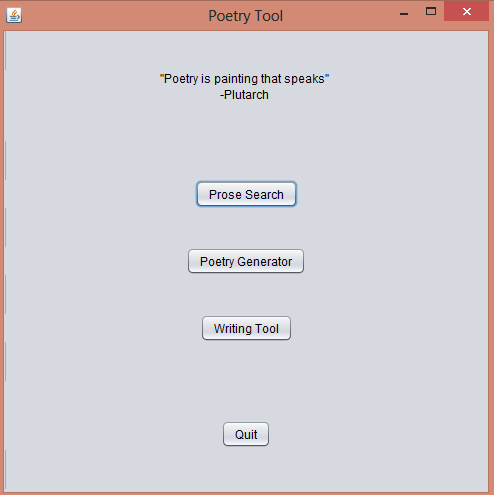
\includegraphics[scale=0.5]{Images/screen1}
    \caption{Main menu of our application}
  \label{screen1}
\end{figure}

\begin{figure}[ht]
  \centering
    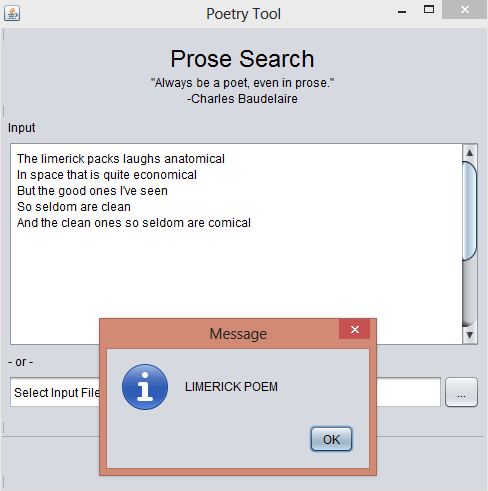
\includegraphics[scale=0.5]{Images/screen2}
    \caption{Recognition Element}
  \label{screen2}
\end{figure}

We also have an UI in place for the generator tool. Presently, we are able to choose a text file (or the corpus of interest) for generating the poem, and we have in place a selection option for the user to choose the type of poetry he/she wants to generate. Of course, depending on the poetry, we also add additional options for the user to play around with (haikus, limericks and couplets are pretty strict, whereas quatrains are not). The UI for the generator component is presented in Figures \ref{screen3} to \ref{screen5}.

\begin{figure}[ht]
  \centering
    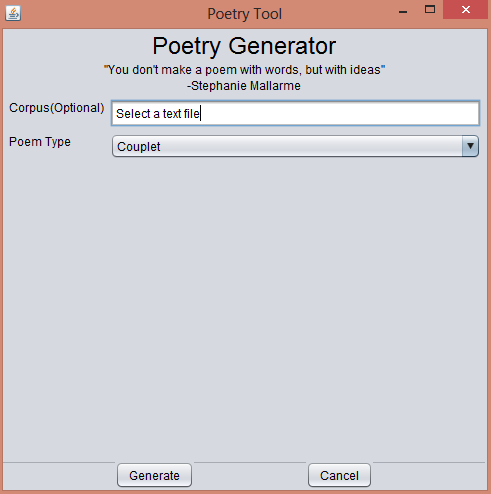
\includegraphics[scale=0.5]{Images/screen3}
    \caption{Poem Generator Window}
  \label{screen3}
\end{figure}

\begin{figure}[ht]
  \centering
    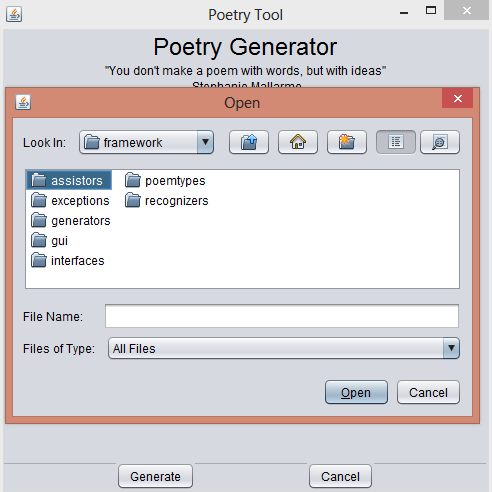
\includegraphics[scale=0.5]{Images/screen5}
    \caption{Choosing an input file}
  \label{screen4}
\end{figure}

\begin{figure}[ht]
  \centering
    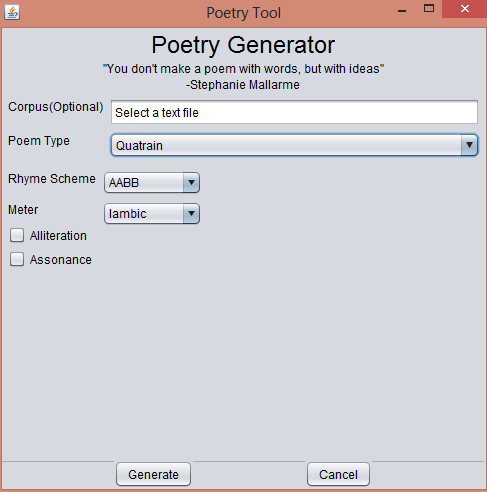
\includegraphics[scale=0.5]{Images/screen4}
    \caption{Customizable options for the user}
  \label{screen5}
\end{figure}



\section*{Description of the Demo}
In the demo, we present the user interface of our application and demo the poetry tool for different input texts and show how they are classified according to the recognition element.

We also have a brief interface overview of the generator tool (we are yet to implement the underlying functionality).

Our code is publicly visible and is located at: \url{https://github.com/arv100kri/Poetry_Framework}

\section*{Architectural Changes from Deliverable 2}

We do not have any significant deviations from the architecture we proposed in Deliverable 2. There is probably one minor “change” at this point - we do not have a central \textbf{\textit{Rule Engine}} as of now. We instead have classes for each category of poems, and each of those classes have rules contained within them. However, when we will have to deal with more difficult/complex types of poems like sonnets etc., we will create this \textbf{\textit{Rule Engine}}.

\section*{Problems faced (and Expected to face)}

It is easy to categorize something if the categories are well defined and disjoint. In case of poems, some types of poetry are fairly easy to identify. A good example is that of limericks that have a fixed rhyme scheme and line count. With other types of poetry, the rhyme scheme may not necessarily be defined and the number of lines may be variable. This makes categorization difficult. We faced this issue in trying to build a generic system that could identify poems using the same functions and had to subsequently limit the categories that our system would recognize. Also, we were forced to write separate modules for recognizing different categories.

Another issue came the in form of limitations with respect to the CMUDict; we assumed that the list of symbols that follow a word correspond to the syllables of the word. However, it turns out that they are actually the syllables alongwith the phoneme representation of them. We are unable as of now to accomplish this in Java. We utilized Python’s NLTK to tokenize the CMUDict and obtain the number of syllables for a given word. Then we used Java’s \textbf{\textit{Runtime}} class to call this Python script and parsed its output into a useable form. Also, since we are using Java, this is probably the fastest way to access the functionalities provided by the rich NLTK library! Of course, we are still exploring alternative ways to hook-up Java with NLTK-like libraries.

We also have to think about implementing contingency methods for certain words, in case they are not present in the CMUDict (which is a very good possibility when analyzing Wikipedia text).

\subsection*{The Future}
\begin{itemize}
    \item The system has hooks for poetry generation, recognition from a corpus, and poetry writing assistance, which need to be implemented.
    \item We have compiled a list of 20 types of poems and their associated attributes. We will try to expand the recognition element to incorporate these types as well.
    \item CMU dictionary also provides syllable and stress information, which we need to leverage in future implementations.
    \item Extend the generate rhyming words module to return a list of words which not only rhyme with the given input word, but are also related to the context (which could be the theme of the poem, or potentially anything else that is useful).
\end{itemize}

\bibliographystyle{unsrt}
\bibliography{myrefs}
\end{document}